% ============================================================
%  Exercise 6 -- NAND Gate Sleep-Mode Leakage Analysis
%  1-page landscape handout, 2 slide boxes (numbered 9--10)
%  Continues from Exercise 5 presentation (boxes 1--8)
%
%  HOW TO COMPILE ON OVERLEAF:
%  Upload this file.  No external images required -- all
%  visuals are generated with TikZ.
% ============================================================
\documentclass[a4paper,landscape,11pt]{article}
\usepackage[utf8]{inputenc}
\usepackage{graphicx}
\usepackage{amsmath}
\usepackage{geometry}
\usepackage{tikz}
\usepackage{booktabs}
\usepackage{helvet}
\usepackage{xcolor}

\renewcommand{\familydefault}{\sfdefault}

\geometry{margin=1cm}

% ---- Slide box (same as Ex 5) ----
\newcommand{\slidebox}[2]{%
    \begin{tikzpicture}
        \draw[thick] (0,0) rectangle (13.5, 8.5);
        \node[anchor=north west, inner sep=0pt, yshift=-5pt] at (0,0) {\footnotesize #1};
        \clip (0.1,0.1) rectangle (13.4,8.4);
        \node[anchor=center] at (6.75, 4.25) {
            \begin{minipage}{12.5cm}
                #2
            \end{minipage}
        };
    \end{tikzpicture}%
}

% ---- Heat-map colour definitions ----
\definecolor{hm0}{HTML}{1B7837}   % deep green   (< 0.001 nA)
\definecolor{hm1}{HTML}{7FBC41}   % light green  (0.001 nA range)
\definecolor{hm2}{HTML}{FEE08B}   % yellow       (0.003–0.013 nA)
\definecolor{hm3}{HTML}{FC8D59}   % orange       (0.06 nA)
\definecolor{hm4}{HTML}{D73027}   % red          (1–12+ nA)

\begin{document}
\pagestyle{empty}

% ==================== PAGE (Exercise 6) ====================

% ---- Box 9 : Leakage Current Summary Table ----
\noindent
\slidebox{9}{
    \centering
    \textbf{Sleep-Mode Leakage \textemdash{} CMOS 2-Input NAND, 22\,nm PTM-HP}\\[0.2cm]
    \scriptsize
    \begin{tabular}{@{}l l l l@{}}
        \toprule
        & \multicolumn{3}{c}{\textbf{Circuit Topology}} \\
        \cmidrule(l){2-4}
        & \textbf{B}\;(PMOS HVT header)
        & \textbf{C}\;(NMOS HVT footer)
        & \textbf{D}\;(header + footer) \\
        \midrule
        Sleep signal & $S = V_{DD}$\;(header OFF) & $\overline{S} = 0$\;(footer OFF) & Both OFF \\
        HVT $V_T$    & $1.5\times$ nominal        & $1.5\times$ nominal               & $1.5\times$ nominal \\
        \bottomrule
    \end{tabular}\\[0.25cm]
    \small
    \begin{tabular}{@{}c r r r r@{}}
        \toprule
        \textbf{Input (AB)} & \textbf{Ckt\,A (nA)} & \textbf{Ckt\,B (nA)} & \textbf{Ckt\,C (nA)} & \textbf{Ckt\,D (nA)} \\
        \midrule
        00 &  0.0607  & 0.00817 & 0.01271 & 0.000960 \\
        01 &  1.027   & 0.00765 & 0.00999 & 0.000642 \\
        10 &  4.144   & 0.00781 & 0.01115 & 0.000466 \\
        11 & \textbf{12.122}  & 0.00282 & 0.01131 & \textbf{0.000102} \\
        \bottomrule
    \end{tabular}\\[0.15cm]
    \flushleft\scriptsize
    $\bullet$\;Leakage = $|I_{DD}|$ from Spectre DC operating-point analysis (nested sweep of A, B).\\
    $\bullet$\;Circuit\,A leakage spans $200\times$ across input states; Circuits B--D are nearly flat.\\
    $\bullet$\;Circuit\,D uses tightened convergence: \texttt{gmindc=1e-15, iabstol=1e-15, reltol=1e-4}.
}
\hfill
% ---- Box 10 : TikZ Heat Map with original nA values ----
\slidebox{10}{
    \centering
    \textbf{Leakage Heat Map \textemdash{} $|I_{DD}|$ (nA)}\\[0.15cm]
    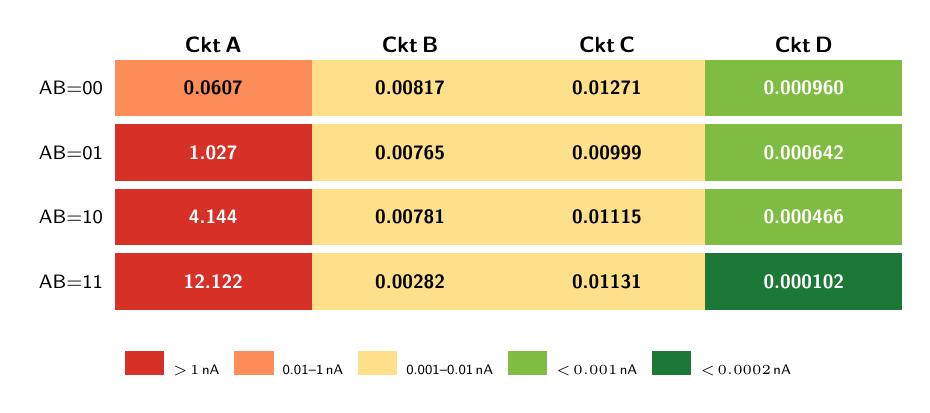
\begin{tikzpicture}[
        cell/.style={minimum width=2.5cm, minimum height=0.72cm,
                     font=\sffamily\bfseries\scriptsize, inner sep=1pt},
        cellw/.style={cell, text=white},
        cellk/.style={cell, text=black},
        lbl/.style={font=\sffamily\scriptsize, minimum width=1.1cm,
                    minimum height=0.72cm, inner sep=2pt, anchor=east}
    ]
    % Column headers
    \node[font=\sffamily\footnotesize\bfseries] at (1.25, 0.55) {Ckt\,A};
    \node[font=\sffamily\footnotesize\bfseries] at (3.75, 0.55) {Ckt\,B};
    \node[font=\sffamily\footnotesize\bfseries] at (6.25, 0.55) {Ckt\,C};
    \node[font=\sffamily\footnotesize\bfseries] at (8.75, 0.55) {Ckt\,D};

    % ---- Row 1: AB = 00 ----
    \node[lbl] at (0, 0) {AB=00};
    \node[cellk, fill=hm3] at (1.25, 0)  {0.0607};
    \node[cellk, fill=hm2] at (3.75, 0)  {0.00817};
    \node[cellk, fill=hm2] at (6.25, 0)  {0.01271};
    \node[cellw, fill=hm1] at (8.75, 0)  {0.000960};

    % ---- Row 2: AB = 01 ----
    \node[lbl] at (0, -0.82) {AB=01};
    \node[cellw, fill=hm4] at (1.25, -0.82)  {1.027};
    \node[cellk, fill=hm2] at (3.75, -0.82)  {0.00765};
    \node[cellk, fill=hm2] at (6.25, -0.82)  {0.00999};
    \node[cellw, fill=hm1] at (8.75, -0.82)  {0.000642};

    % ---- Row 3: AB = 10 ----
    \node[lbl] at (0, -1.64) {AB=10};
    \node[cellw, fill=hm4] at (1.25, -1.64)  {4.144};
    \node[cellk, fill=hm2] at (3.75, -1.64)  {0.00781};
    \node[cellk, fill=hm2] at (6.25, -1.64)  {0.01115};
    \node[cellw, fill=hm1] at (8.75, -1.64)  {0.000466};

    % ---- Row 4: AB = 11 ----
    \node[lbl] at (0, -2.46) {AB=11};
    \node[cellw, fill=hm4] at (1.25, -2.46)  {12.122};
    \node[cellk, fill=hm2] at (3.75, -2.46)  {0.00282};
    \node[cellk, fill=hm2] at (6.25, -2.46)  {0.01131};
    \node[cellw, fill=hm0] at (8.75, -2.46)  {0.000102};

    % ---- Colour legend ----
    \node[font=\sffamily\tiny, anchor=west] at (0, -3.5) {%
        \tikz{\node[fill=hm4, minimum width=0.5cm, minimum height=0.3cm] {};}
        \;$>\!1$\,nA\quad
        \tikz{\node[fill=hm3, minimum width=0.5cm, minimum height=0.3cm] {};}
        \;0.01--1\,nA\quad
        \tikz{\node[fill=hm2, minimum width=0.5cm, minimum height=0.3cm] {};}
        \;0.001--0.01\,nA\quad
        \tikz{\node[fill=hm1, minimum width=0.5cm, minimum height=0.3cm] {};}
        \;$<\!0.001$\,nA\quad
        \tikz{\node[fill=hm0, minimum width=0.5cm, minimum height=0.3cm] {};}
        \;$<\!0.0002$\,nA%
    };
    \end{tikzpicture}\\[0.1cm]
    \flushleft\scriptsize
    $\bullet$\;All values in nA.  Colour encodes leakage magnitude on a logarithmic scale.\\
    $\bullet$\;Circuit\,A spans 4 decades (red$\to$orange); B\,\&\,C collapse to a narrow yellow band; D reaches green.
}

\end{document}
